%\begin{savequote}[8cm]
%\textlatin{Jedem Anfang wohnt ein Zauber innne.}
%
%In the core of every beginning lives magic.
%  \qauthor{--- Hermann Hesse's \textit{Stufen}}
%\end{savequote}

\chapter{\label{ch:2-background}Theoretical Background} 

%\minitoc

\section{Introduction}
This chapter describes the theoretical background of machine learning and counterfactual inference including their formalisation, core concepts, state-of-the-art, and challenges. 

We start by giving a general introduction to machine learning and  its core concepts. 

The second part of the chapter deals with  \emph{deep learning} -- a particular subset of machine learning that uses deep neural networks. 

The last part of the chapter is dedicated to the problem of counterfactual inference. We describe the importance of the problem and its application areas, and give a formalisation. Furthermore, we outline the challenges of the problem and the different approaches that have been applied to it so far. We conclude, by relating counterfactual inference to deep learning and describing its open research questions which is the very foundation of this thesis. 

% TODO Intro: Write introduction in more detail depending on the actual contents. 


\section{Machine Learning}


\subsection{Motivation}
When conceptualising computer programs, we often think of them as series of unambiguous, (mostly) atomic instructions that are executed in a deterministic way and have to be explicitly programmed by a human programmer. 

While certain problem areas -- in particular those for which a well-defined algorithm or effective step-by-step solution strategy exists -- can successfully expressed and ultimately solved this way, there are various problems where this seems infeasible. A typical example for the second category is autonomous driving for which there are far too many situations and eventualities to encode the desired behaviour of an autonomous vehicle as a finite sequence of conditional instructions. 

Machine learning is a subfield of computer science that deals with the question of how to teach computer programs to learn without being explicitly programmed what to do. 
% TODO Check if this it too close to the quote at wikipedia 

More formally, an algorithm "is said to learn from experience E with respect to some class of tasks T and performance measure P if its performance at tasks in T, as measured by P, improves with experience E". (Mitchell)
% CITE:  Mitchell, T. (1997). Machine Learning. McGraw Hill. p. 2. ISBN 0-07-042807-7.
Recalling our example of autonomous driving, for instance, we could define the task $T$ in terms of "moving the car from A to B" while our performance measure $P$ might include aspects such as the travel time and the number of people or objects harmed. The experience $E$ would consists of the \emph{training data} that is acquired by previously covered distances (either autonomously or by "observing" a human driver). 

% TODO Show diagram (model, algorithm, learning, data)

\subsection{Types of Learning}
Machine Learning is typically categorised into \emph{supervised learning}, \emph{unsupervised learning}, \emph{reinforcement learning}. 

% TODO For each of the categories, make it more formal 

\subsubsection{Supervised Learning} 
In supervised learning the task is to infer a function over a number of samples from a set of training data that is said to be \emph{labelled}. In other words, for each sample in the training data, we have access to the actual function value we want to predict. 

For instance, we might be interested predicting housing prices where we are given a dataset consisting of historic information regarding houses (e.g. number of rooms, area in $m^2$, etc.), commonly referred  to as \emph{features} or \emph{covariates}, and the actual price for which the house has been sold, called \emph{outcome}, \emph{target}, or \emph{label}. Once a certain model has been trained by using the historic labelled dataset, we can use the same model to predict the housing prices on unseen data points, i.e. new houses for which the price is unknown. Such a task of predicting a continuous variable is called a \emph{regression} task whereas the predicting of a discrete output is referred to as a \emph{classification} task. 

\subsubsection{Unsupervised Learning} 
In contrast to supervised learning, the training set in an unsupervised setting does not contain the target labels. Typical tasks in this field include finding particular patterns in the data and clustering it accordingly. It is important to note, however, that for supervised learning, there is normally no ground-truth meaning that the performance (or quality) of the outcome cannot be easily be measure or even defined in absolute terms but might depend on the underlying use-case of the clustering. Another important task in supervised learning is \emph{dimensionality reduction} for which a (in terms of the features) high-dimensional dataset is reduces to a target lower dimension while trying to minimise the information loss. 

\subsubsection{Reinforcement Learning}
In reinforcement learning, a software agent has to learn appropriate actions in a dynamic environment in which the consequences of an action might not be immediately accessible but add up to a long-term reward that ought to be maximised. 

A most prominent example was mentioned earlier with the task of autonomous driving in which a vehicle is governed by a piece of software that has to find adequate series of actions (steering, regulating speed, etc.) in order to reach a target destination in a complex and ever-changing environment. 


% TODO! Re-create graph!
\begin{figure}[]
	\label{fig:machine-learning-approach}
	\caption{Schematic Approach of Machine Learning. A selected model $M$ is trained on a dataset $D$ using a learning algorithm $A$.}
	\centering
	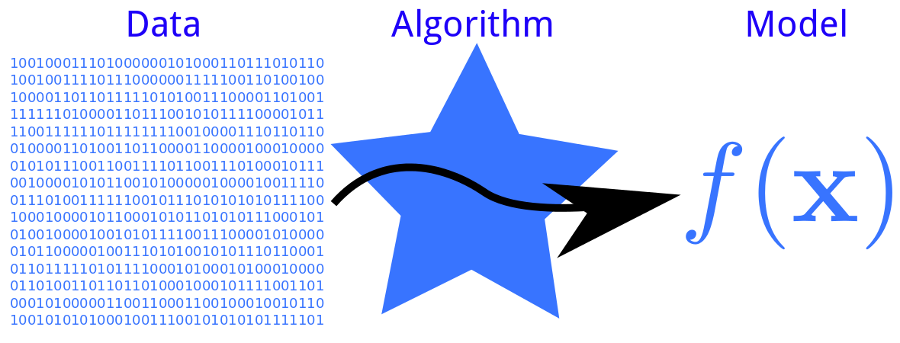
\includegraphics[width=0.5\textwidth]{figures/chapter-2/machine-learning-approach.png}
\end{figure}
\subsection{Machine Learning Models}
As illustrated in figure \ref{fig:machine-learning-approach}, machine learning is based on the concept of selecting an appropriate model and fitting it to a given (training) data set using a training algorithm. 

For instance, we might want to use a \emph{linear model} for our task of predicting housing prices. We can then make use \emph{linear regression} which allows us to fit our linear model to our labelled dataset of existing houses and their prices. 
 
The selection of an appropriate model is of great importance and determines important factors such as the trade-off between the expressiveness (i.e. the ability to capture complex relationships) and the computational complexity of our model (i.e. how difficult it is to train it). 

There is a number of models each with individual pros and cons depending on the desired task and the desired characteristics. Typical models include \emph{linear models}, \emph{decision trees}, and \emph{neural networks}. 
% TODO What are other typical models. How do they compare against each other? 
% Should I sketch them out here? 

This dissertation focuses on using \emph{deep learning} for the problem of counterfactual inference. Therefore, a dedicated part of this chapter deals exclusively with deep neural networks and describes their characteristics in more detail. 



%\subsection{Training}
%Machine learning is based on the concept of training a selected model by using a 
%
%Typically: Gradient Descent
%
%
%What types are there? 
%What's the challenge? (local minimum, symmetries, etc.)
%% TODO Include graph

\subsection{Regularisation}
When training our model we have to find the right balance between fitting it most accurately to the training data while making sure that the model generalises will for unseen data points. 
Given that the expressiveness of the model is sufficiently high to capture it, we might naively fit our model to the training data perfectly, resulting in a training error of zero. This, however, would merely "memorise" the training data and might perform poorly on unseen future data points. This phenomenon where we overfit the training data is often referred to as \emph{high variance}. 
In contrast, if the model is too simple, we night not be able to accurately capture the relationship in our data leading to equally poor results. In this case, we are under-fitting the data and our model has a so called \emph{high bias}.
Therefore, the goal is to train the model in a way that neither overfits nor underfits and generalises well to unseen datapoints. This can be achieved by a concept called \emph{regulariation}.  

% TODO! Re-create graph!
\begin{figure}[]
	\label{fig:overfitting-underfitting}

	\centering
	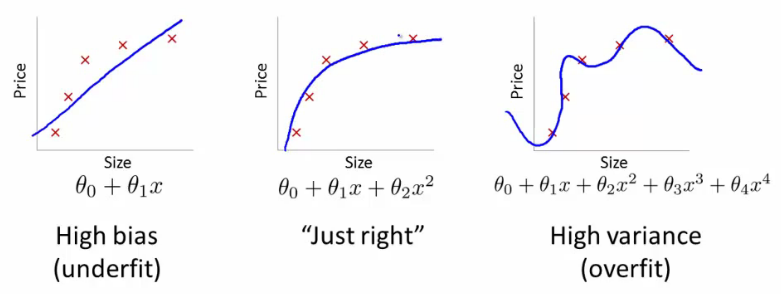
\includegraphics[width=0.8\textwidth]{figures/chapter-2/overfitting-underfitting.png}
	\caption{Visualisation of Bias variance Tradeoff. The model on the left is ... whereas the middle one ... and the right one is ...}
\end{figure}

% TODO Should I include learning curves as well? 
%% TODO! Re-create graph!
%\begin{figure}[]
%	\label{fig:machine-learning-approach}
%	\caption{Visualisation of Learning Curves. The left model is ... whereas the right model is ...}
%	\centering
%	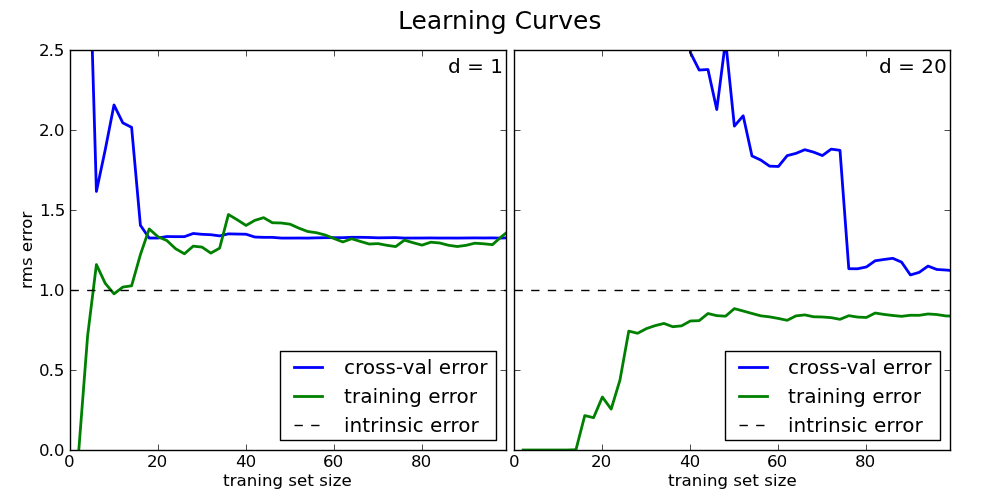
\includegraphics[width=0.8\textwidth]{figures/chapter-2/learning-curves.png}
%\end{figure}




\section{Deep Learning}
\subsection{Motivation}
Lorem ipsum dolor sit amet consectetur, adipiscing elit mus neque montes, suspendisse et sociis vestibulum.

\subsection{The Perceptron}
Lorem ipsum dolor sit amet consectetur, adipiscing elit mus neque montes, suspendisse et sociis vestibulum.

\subsection{Multi-Layer-Perceptron}
Lorem ipsum dolor sit amet consectetur, adipiscing elit mus neque montes, suspendisse et sociis vestibulum.

\subsection{Training}
Lorem ipsum dolor sit amet consectetur, adipiscing elit mus neque montes, suspendisse et sociis vestibulum.

\subsection{Types and Topologies}
Lorem ipsum dolor sit amet consectetur, adipiscing elit mus neque montes, suspendisse et sociis vestibulum.

\subsection{Multi-Task Learning}
Lorem ipsum dolor sit amet consectetur, adipiscing elit mus neque montes, suspendisse et sociis vestibulum.

\subsection{Hyper-paramaters}
Lorem ipsum dolor sit amet consectetur, adipiscing elit mus neque montes, suspendisse et sociis vestibulum.

\subsection{Challenges}
Lorem ipsum dolor sit amet consectetur, adipiscing elit mus neque montes, suspendisse et sociis vestibulum.


\section{Counterfactual Inference}
\subsection{Motivation}
Lorem ipsum dolor sit amet consectetur, adipiscing elit mus neque montes, suspendisse et sociis vestibulum.

\subsection{Formalisation}
Lorem ipsum dolor sit amet consectetur, adipiscing elit mus neque montes, suspendisse et sociis vestibulum.

\subsection{Counterfactual Inference vs. Supervised Learning}
Lorem ipsum dolor sit amet consectetur, adipiscing elit mus neque montes, suspendisse et sociis vestibulum.

\subsection{Propensity Score}
Lorem ipsum dolor sit amet consectetur, adipiscing elit mus neque montes, suspendisse et sociis vestibulum.

\subsection{Status Quo}
Lorem ipsum dolor sit amet consectetur, adipiscing elit mus neque montes, suspendisse et sociis vestibulum.

\subsection{Open Questions}
Lorem ipsum dolor sit amet consectetur, adipiscing elit mus neque montes, suspendisse et sociis vestibulum.

